\newpage

% Since the transformation method given in question 4 is only valid for natural values of the shape parameters, we will often rely on an Accept-Reject algorithm to sample values from a more general beta distribution.

\section{In the case where $\alpha$ and $\beta$ are larger than 1 (but not necessarily natural numbers), it is possible to use the uniform distribution $\mathcal{U}[0, 1]$ as instrumental distribution.}

% -------------------------------------------------------------------------------------------------

\subsection*{(a) Explain why this is possible and how to determine the limiting constant $C$.}

In the Accept–Reject (A–R) algorithm, the target density \(f\) can be sampled using an instrumental density \(g\) if there exists a constant \(C \geq 1\) such that:
\begin{equation}
f(x) \leq C g(x) \quad \forall x \in \operatorname{supp}(f)
\end{equation}

For the Beta distribution \(\text{Be}(\alpha, \beta)\) with \(\alpha > 1\) and \(\beta > 1\), the probability density function is:
\begin{equation}
f(x) = \frac{1}{B(\alpha, \beta)} x^{\alpha - 1} (1 - x)^{\beta - 1}, \quad x \in [0, 1]
\end{equation}
This density is smooth, unimodal, and bounded on \([0,1]\). Hence, the uniform distribution \(\mathcal{U}[0,1]\) is a natural choice for the instrumental distribution because:
\begin{itemize}
    \item It shares the same support, \([0,1]\).
    \item Its density is constant: \(g(x) = 1\).
\end{itemize}

With \(g(x) = 1\), the density ratio simplifies to:
\begin{equation}
\frac{f(x)}{g(x)} = f(x)
\end{equation}
and the limiting constant becomes:
\begin{equation}
C = \sup_{x \in [0, 1]} f(x)
\end{equation}

When \(\alpha > 1\) and \(\beta > 1\), the mode of the Beta distribution lies strictly inside \((0,1)\) and is given by:
\begin{equation}
x_{\text{mode}} = \frac{\alpha - 1}{\alpha + \beta - 2}
\end{equation}
Therefore, \(C\) can be computed by evaluating the Beta PDF at the mode:
\begin{equation}
C = f(x_{\text{mode}}) = \frac{1}{B(\alpha, \beta)} \left(\frac{\alpha - 1}{\alpha + \beta - 2}\right)^{\alpha - 1} \left(1 - \frac{\alpha - 1}{\alpha + \beta - 2}\right)^{\beta - 1}
\end{equation}


% In the Accept–Reject (AR) algorithm, we sample from a target density $f(x)$ by using a simpler instrumental distribution $g(x)$, provided that:
% \[
% \frac{f(x)}{g(x)} \leq C, \quad \forall x \in \text{supp}(f),
% \]
% where $C$ is a finite constant and $g(x)$ is easy to sample from.

% For the Beta distribution $\text{Be}(\alpha, \beta)$ with $\alpha > 1$ and $\beta > 1$, the probability density function is:
% \[
% f(x) = \frac{1}{B(\alpha, \beta)} x^{\alpha - 1} (1 - x)^{\beta - 1}, \quad x \in [0, 1].
% \]
% This density is smooth, unimodal, and bounded. Therefore, we can safely use the uniform distribution $\mathcal{U}[0,1]$ as the instrumental distribution since:
% \begin{itemize}
%     \item It shares the same support $[0, 1]$
%     \item Its density is constant: $g(x) = 1$
% \end{itemize}

% With $g(x) = 1$, the density ratio simplifies to:
% \[
% \frac{f(x)}{g(x)} = f(x),
% \]
% and the limiting constant becomes:
% \[
% C = \sup_{x \in [0, 1]} f(x).
% \]

% When $\alpha > 1$ and $\beta > 1$, the mode of the Beta distribution is located at:
% \[
% x_{\text{mode}} = \frac{\alpha - 1}{\alpha + \beta - 2}.
% \]
% Therefore, instead of evaluating the PDF over a full grid, we can compute the limiting constant more directly as:
% \[
% C = f(x_{\text{mode}}) = \frac{1}{B(\alpha, \beta)} \left(\frac{\alpha - 1}{\alpha + \beta - 2}\right)^{\alpha - 1}
% \left(1 - \frac{\alpha - 1}{\alpha + \beta - 2}\right)^{\beta - 1}.
% \]

% This approach is exact (when applicable) and computationally efficient. It also reflects the probabilistic interpretation of the mode as the value most likely to be drawn from the Beta distribution.





% \textit{Note: This formula for the mode and thus for \(C\) applies only when \(\alpha > 1\) and \(\beta > 1\), since only then does the mode lie strictly within \((0,1)\). For other parameter values (e.g., \(\alpha \leq 1\) or \(\beta \leq 1\)), the Beta PDF attains its maximum at the boundaries \(x=0\) or \(x=1\), and \(C\) must be computed accordingly.}



% --- 1st draft

% In the Accept–Reject (AR) method, we aim to sample from a target density $f(x)$ using a simpler instrumental density $g(x)$ such that:
% \[
% f(x) \leq C g(x), \quad \forall x \in \text{supp}(f),
% \]
% where $C > 0$ is the \textit{limiting constant} ensuring that the ratio $f(x)/g(x)$ is bounded.

% In the case of a Beta distribution $\text{Be}(\alpha, \beta)$ with $\alpha > 1$ and $\beta > 1$, the density function is:
% \[
% f(x) = \frac{1}{B(\alpha, \beta)} x^{\alpha - 1} (1 - x)^{\beta - 1}, \quad x \in [0, 1].
% \]

% This function is:
% \begin{itemize}
%     \item Smooth and continuous on $[0,1]$
%     \item Unimodal, with a well-defined maximum when $\alpha, \beta > 1$
%     \item Finite and bounded, as there are no singularities at 0 or 1
% \end{itemize}

% Therefore, it is valid to use the uniform distribution $\mathcal{U}[0,1]$ as the instrumental distribution, since it:
% \begin{itemize}
%     \item Has the same support as the Beta distribution: $[0, 1]$
%     \item Has a constant density: $g(x) = 1$
% \end{itemize}

% Under this choice, the density ratio becomes:
% \[
% \frac{f(x)}{g(x)} = f(x)
% \]
% which is bounded on $[0, 1]$. Hence, the limiting constant $C$ is simply the supremum of $f(x)$:
% \[
% C = \sup_{x \in [0, 1]} f(x)
% \]

% This maximum can be determined numerically, for example, by evaluating the Beta density on a fine grid of points in $[0,1]$. Once $C$ is known, it can be used to define the acceptance criterion in the Accept–Reject sampling algorithm.




% --- reference

% \[
% \frac{f(x)}{g(x)} \leq C
% \]

% Since the PDF of a uniform $(0, 1)$ is equal to 1, the limiting constant is the maximum value of the PDF of the target distribution (here, the beta distribution). This value can be evaluated at the mode of the beta distribution; it corresponds to the value that has the highest probability to be drawn. The mode is given by 
% \[
% \frac{\alpha - 1}{\alpha + \beta - 2}.
% \]
% Therefore, the limiting constant can be calculated using this formula:
% \[
% C = f\left(\frac{\alpha - 1}{\alpha + \beta - 2}\right)
% \]





% -------------------------------------------------------------------------------------------------
\newpage
\subsection*{(b) Determine (using R) this limiting constant $C$ used in the Accept-Reject algorithm if the target distribution is $\text{Be}(3.3, 9.5)$.}

To apply the Accept–Reject algorithm with the uniform instrumental distribution \(\mathcal{U}[0, 1]\), the constant \(C\) must satisfy:
\begin{equation}
\frac{f(x)}{g(x)} \leq C, \quad \forall x \in [0, 1]
\end{equation}
where \(f(x)\) is the Beta PDF and \(g(x) = 1\).

For \(\alpha > 1\) and \(\beta > 1\), the maximum of \(f(x)\) occurs at the mode:
\begin{equation}
x_{\text{mode}} = \frac{\alpha - 1}{\alpha + \beta - 2}
\end{equation}

Substituting \(\alpha = 3.3\) and \(\beta = 9.5\) yields:
\[
x_{\text{mode}} = \frac{3.3 - 1}{3.3 + 9.5 - 2} = \frac{2.3}{10.8} \approx 0.213
\]

The limiting constant is then:
\[
C = f(x_{\text{mode}}) = \frac{1}{B(3.3, 9.5)} \cdot (0.213)^{2.3} \cdot (1 - 0.213)^{8.5}
\]

Numerical evaluation gives:
\[
C \approx 3.3681
\]


% This value serves as the upper bound for the ratio $f(x)/g(x)$ and is used in the acceptance criterion of the Accept–Reject algorithm.



% ---

% Evaluating the beta pdf at its mode, we have $C \approx 3.5864$.

% -------------------------------------------------------------------------------------------------

\subsection*{(c) Implement the algorithm and perform 15,000 simulations to obtain values from a $\text{Be}(3.3, 9.5)$ distribution.}

To simulate values from a $\text{Be}(3.3, 9.5)$ distribution, we implemented the Accept–Reject algorithm using the uniform distribution $\mathcal{U}[0, 1]$ as the instrumental distribution and a limiting constant $C \approx 3.3681$ (computed in part (b)).

The procedure is as follows:
\begin{enumerate}
    \item Sample $x \sim \mathcal{U}[0, 1]$.
    \item Sample $u \sim \mathcal{U}[0, 1]$.
    \item Accept $x$ if $u < \frac{f(x)}{C}$, where $f(x)$ is the Beta density.
    \item Repeat until 15,000 accepted values are obtained.
\end{enumerate}

In total, we simulated values until 15,000 accepted samples were obtained.

% -------------------------------------------------------------------------------------------------
\newpage
\subsection*{(d) Create a plot that shows all simulated values, distinguishing between the accepted (in green) and rejected values (in red). Also indicate the instrumental density and the true density function of the $\text{Be}(3.3, 9.5)$ distribution. Calculate the acceptance rate.}

The results of the Accept–Reject simulation from part (c) are visualized in the figure below. We distinguish between:
\begin{itemize}
    \item Accepted samples shown in green, these follow the target $\text{Be}(3.3, 9.5)$ distribution.
    \item Rejected proposals shown in red, these are the values that did not satisfy the acceptance criterion.
\end{itemize}

\begin{figure}[H]
    \centering
    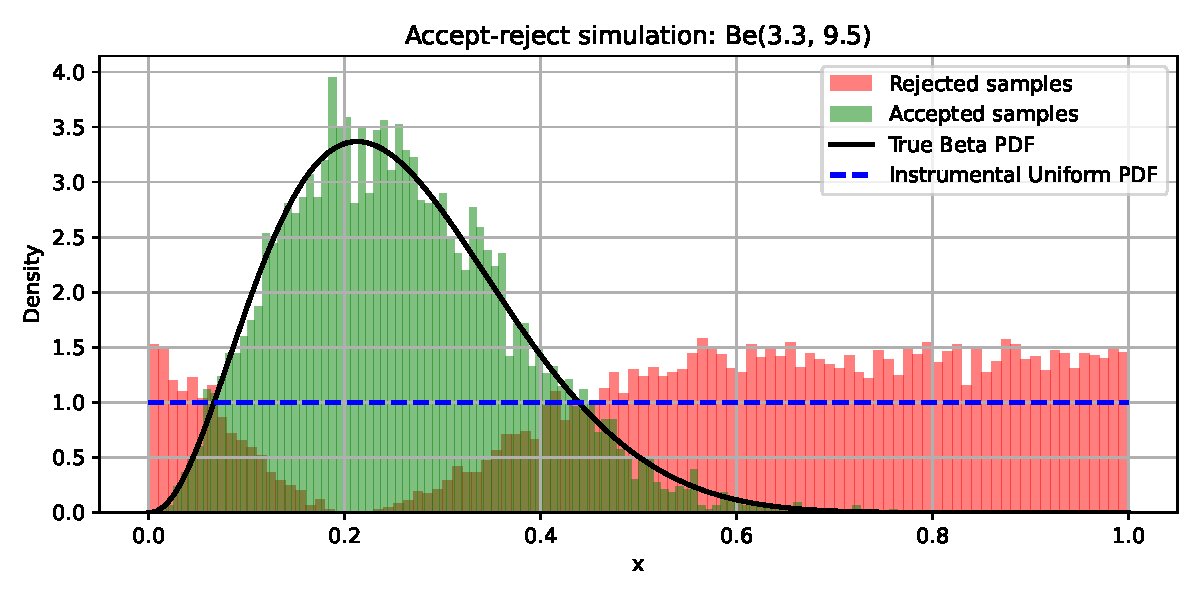
\includegraphics[width=0.7\textwidth]{resources/figures/q7d-beta_accept_reject.pdf}
    \noskipcaption{Accepted and rejected samples with uniform distribution as instrumental density (15,000 samples).}
    \label{fig:q7d}
\end{figure}

We observe from Figure~\ref{fig:q7d} that accepted values are concentrated around the mode of the Beta distribution (approximately $x \approx 0.213$), while rejected values are more common in low-density tail regions.

\medskip
The empirical acceptance rate was calculated as:
\[
\text{Acceptance rate} = \frac{\text{\# accepted}}{\text{\# accepted} + \text{\# rejected}} = \frac{\text{\# accepted}}{15,\!000} \approx 29.37\%
\]

% This value is consistent with theoretical expectations given the limiting constant $C \approx 3.3681$.





% The graph obtained after running the algorithm is displayed in the following figure:

% \begin{figure}[h]
%     \centering
%     % \includegraphics[width=0.8\textwidth]{your-figure-file.pdf} % Replace with actual file name
%     \caption{Accept-Reject algorithm for beta distribution with uniform distribution as instrumental density (10,000 samples).}
%     \label{fig:accept-reject}
% \end{figure}

% The acceptance rate can be calculated as the ratio between the accepted values divided by the sum of the accepted values and the rejected ones.

% \[
% \text{Acceptance rate} = \frac{\text{Nb of accepted values}}{\text{Nb of accepted values} + \text{Nb of rejected values}}
% \]

% Which is 0.2745 in our case.



% -------------------------------------------------------------------------------------------------
\newpage
\subsection*{(e) Show, in a general setting, that the probability of acceptance in an Accept-Reject algorithm with limiting constant $C$ on the density ratio $f/g$ is equal to $1/C$. Compare this result with the calculated value in the previous question.}

Consider the Accept–Reject method where:

\begin{itemize}
    \item \(f(x)\) is the target density.
    \item \(g(x)\) is the instrumental (proposal) density.
    \item There exists a constant \(C \geq 1\) such that:
    \begin{equation}
    f(x) \leq C g(x), \quad \forall x
    \end{equation}
    \item \(X \sim g\) and \(U \sim \mathcal{U}[0,1]\) are independent.
\end{itemize}

Define the acceptance event as:
\begin{equation}
A := \left\{ U \leq \frac{f(X)}{C g(X)} \right\}
\end{equation}

The probability of acceptance is:
\begin{equation}
P(A) = \mathbb{E}_X \left[ P\left(U \leq \frac{f(X)}{C g(X)} \mid X \right) \right]
\end{equation}

Since \(U\) is uniform on \([0,1]\), this inner probability is simply:
\begin{equation}
P\left(U \leq \frac{f(X)}{C g(X)} \mid X \right) = \frac{f(X)}{C g(X)}
\end{equation}

Therefore,
\begin{align}
P(A) &= \int_0^1 \frac{f(x)}{C g(x)} g(x) \, dx \\
&= \frac{1}{C} \int_0^1 f(x) \, dx \\
&= \frac{1}{C}
\end{align}

Since \(f\) is a probability density function, it integrates to 1. Thus, the acceptance probability is exactly the reciprocal of the constant \(C\).

\vspace{1em}
\textbf{Comparison with the Beta simulation:}

From part (b), the limiting constant was computed as $C \approx 3.3681$, which implies a theoretical acceptance probability of:
\[
p_{\text{accept}} = \frac{1}{C} \approx 29.69\%
\]

From the empirical results in part (d), the observed acceptance rate was approximately 29.37\%.

The close agreement between theory and empirical results validates the correctness of the Accept–Reject algorithm and confirms that the expected acceptance rate is \(1/C\).






% ---

% The acceptance probability is defined as being a random variable generated from an instrumental distribution and being accepted. We have
% \[
% P(A) = \int_{-\infty}^{+\infty} P(A \mid X) g(x) dx
% \]

% $A$ being the condition to be accepted. In our case, we accept the sample if the random variable generated from a uniform distribution $(0, 1)$ is less than $M(x)$. Therefore, the probability of acceptance is
% \[
% P(A \mid X) = M(x) = \frac{f(x)}{C g(x)}
% \]

% We can substitute in the integral,
% \[
% P(A) = \int_{-\infty}^{+\infty} \frac{f(x)}{C g(x)} g(x) dx = \frac{1}{C} \int_{-\infty}^{+\infty} f(x) dx
% \]

% $f$ being a density distribution, the integral over its domain is equal to 1. We then have,
% \[
% P(A) = \frac{1}{C}
% \]

% Using the value of $C$ obtained earlier, the acceptance probability is equal to 0.278827438. The acceptance rate obtained is really close to the probability of acceptance. This is because it is an empirical way of estimating the beta distribution.



% -------------------------------------------------------------------------------------------------
\newpage
\subsection*{(f) Rewrite the algorithm to obtain $n = 15,\!000$ simulated (accepted) values from the $\text{Be}(3.3, 9.5)$ distribution. Does this influence the acceptance rate obtained by the Accept-Reject algorithm? Plot the simulated values and compare with the true distribution. Discuss your findings.}

% In this part, we modified the Accept–Reject algorithm to continue sampling until exactly \( n = 15,\!000 \) values were accepted from the \(\text{Be}(3.3, 9.5)\) distribution. This approach ensures a fixed number of simulated values, rather than stopping after a predetermined number of trials.

\medskip
The revised algorithm proceeds as follows:
\begin{enumerate}
    \item Repeat:
    \begin{itemize}
        \item Sample \( x \sim \mathcal{U}[0, 1] \)
        \item Sample \( u \sim \mathcal{U}[0, 1] \)
        \item Accept \( x \) if \( u < \frac{f(x)}{C} \), where \( f(x) \) is the Beta(3.3, 9.5) density and \( C \approx 3.3681 \)
    \end{itemize}
    \item Stop when 15,\!000 accepted values are obtained.
\end{enumerate}

% \subsubsection*{Empirical results and visualization}

The empirical acceptance rate is:
\[
\text{Acceptance rate} = \frac{\text{\# accepted}}{\text{\# accepted} + \text{\# rejected}} = \frac{15,\!000}{15,\!000 + \text{\# rejected}} \approx 29.61\%
\]

This value is nearly identical to the rate observed in part (d), confirming that the process of stopping at exactly 15,\!000 accepted values does not significantly influence the acceptance rate. The theoretical rate remains approximately \( 1/C \approx 29.69\% \), with only minor variation due to stochastic sampling.

\medskip
The Figure~\ref{fig:7f} shows the histogram of the simulated values, compared against the true density of the \(\text{Be}(3.3, 9.5)\) distribution.

\begin{figure}[H]
    \centering
    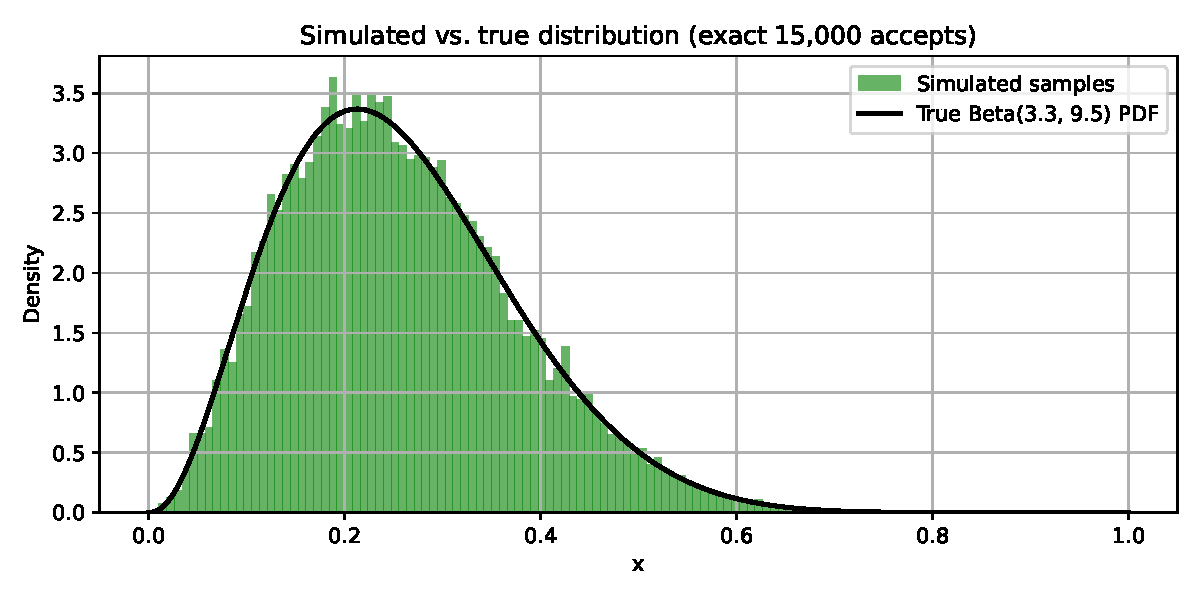
\includegraphics[width=0.7\textwidth]{resources/figures/q7f-beta_fixed_15k_accepts.pdf}
    \noskipcaption{Simulated values and true Beta(3.3, 9.5) PDF.}
    \label{fig:7f}
\end{figure}

% \subsubsection*{Discussion}

The simulated histogram closely follows the true Beta density, with the mode and overall shape accurately reproduced. Fixing the number of accepted samples does not affect the theoretical acceptance rate, which remains approximately \(1/C \approx 29.69\%\). The empirical acceptance rate of approximately \(29.61\%\) confirms the consistency and robustness of the Accept–Reject algorithm under this configuration. 
This approach is practical in applications where a fixed sample size is required regardless of the number of trials.



% ---

% The acceptance rate is now equal to 0.2788389. This value is closer to the theoretical value $\frac{1}{C}$ because we have more accepted samples. This illustrates the law of large numbers: when we increase the number of samples, the representation of the samples becomes more close to the target distribution.

% On the previous question, we generated 10,000 samples, but here, we do have 10,000 accepted samples. Since we will generate 3.586 (value of $C$) samples on average before accepting one, we have a sample size 3.586 times bigger for this question. And therefore, the representation of the beta distribution is better.

% \begin{figure}[h]
%     \centering
%     % \includegraphics[width=0.8\textwidth]{your-figure-file.pdf} % Replace with actual figure file
%     \caption{Accept-Reject algorithm for beta distribution with uniform distribution as instrumental density (10,000 accepted values).}
%     \label{fig:accept-reject-accepted}
% \end{figure}



